% Условная компиляция для самостоятельной работы
\ifdefined\mainfile
    % Если это часть основного файла, не добавляем начало и конец документа
\else
    \documentclass[12pt, a4paper]{report}
    \usepackage{/Users/vladbelousov/Desktop/Semestr_4-FP-NSU/Настройка/library}
    \usepackage[utf8]{inputenc} % Подключение поддержки UTF-8
    \begin{document}
\fi

%%-------------------------------%%

\section{ Вариационная задача с высшими производными }

\[ I[y ]= \int_{x_0 }^{x_1 } F( x, y (x), y' (x),..., y ^{(n )} (x))  dx\]  

\[ \begin{cases}
    y(x_0) = y_0 ,\quad  y (x_1) = y_1 \\
    y ' (x_0) = y ' _0 , \quad y ' (x_1) = y ' _1 \\
    \ldots 
    y^{(n )} = y^{(n )}_0, \quad y^{(n )} (x_1) = y^{(n )}_1
\end{cases} \]  

Необходимое условие локального экстремума: 

Если функция \( \tilde{y }(x ) \)  доставляет функционалу локальному экстремум, то \( \tilde{ y }(x) \)  - решение диффернциального уравнения

\[ \frac{\partial  F }{\partial  y } - \frac{d}{dx } \frac{ \partial  F }{\partial  y ' } + \frac{d ^2 }{dx ^2 } \frac{\partial  F }{\partial  y ''} + \ldots + (-1 )^{n}  \frac{d ^n }{dx ^n } \frac{\partial  F }{\partial  y ^{(n )}} = 0    \] 


\begin{proof}
    \[   \] 
    Пусть \( \tilde{y }( x) \)  доставляет функционалу локальный минимум \( \Rightarrow  \exists \varepsilon_0 >0 , \text{ }  \forall  y(x )\), удовлетворяет краевым условиям, \( \displaystyle \sup_{x \in [x_0 , x_1 ] } |y(x)-\tilde{y }(x) | < \varepsilon_0  \Rightarrow I[\tilde{y }] \le  I[y] \) 

    Возьмем \( y(x ) = \tilde{y }( x ) + \varepsilon \eta ( x ), \eta(x) \)  финитная функция.

    \[ \underbrace{I[\tilde{ y }]}_{g(0)} \le  \underbrace{I[\tilde{y }+ \varepsilon \eta ]}_{g(\varepsilon)} \Rightarrow g(0 ) \le  g(\varepsilon) \Rightarrow \varepsilon = 0  - \text{ точка локального минимума для функции } g(\varepsilon) \] 

    \[ g ' (0 ) = 0 \]  

    \[ 0 = \frac{d}{d \varepsilon } g(\varepsilon ) \bigg |_{\varepsilon = 0 }  = \frac{d}{d \varepsilon} \int_{x_0 }^{x_1} F ( x, \tilde{y }( x)  + \varepsilon \eta ( x ), \tilde{y }' ( x) + \varepsilon \eta' ( x ), ...) dx \bigg |_{\varepsilon = 0} \] 

    Если \( F \in C^{\infty  } (\mathbb{R} ^{n +2 } ), y(x ) \in C^{\infty  } ([x_0 , x_1 ])    \), то 

    \[ 0 = \int_{x_0 }^{x_1} \left[ \frac{\partial  F }{\partial  y } \eta( x) + \frac{\partial F }{\partial  y' }(... )\eta' ( x )+ \frac{\partial F }{\partial y ''} (...) \eta''(x) +\dots  \right]  dx \bigg | _{\varepsilon = 0 }  =    \] 

    \[ =\int_{x_0 }^{x_1}  \frac{\partial  F }{\partial  y } \eta ( x ) dx + \frac{\partial  F } {\partial  y ' } \eta  ( x ) \bigg |_{x_0 }^{x_1}   - \int_{x_0 }^{x_1} \eta( x ) \frac{d }{dx } \frac{\partial  F }{\partial  y ' } (... )dx + \frac{\partial  F }{ \partial  y ' } (... ) \eta ( x ) \bigg |_{x_0 }^{x_1} - \int_{x_0 }^{x_1}  \eta ' ( x ) \frac{d}{dx } \frac{\partial  F }{\partial  y ''} dx ... \text{ и тд}    \] 

    \[ \text{Для n =2:}  \int_{x_0 }^{x_1} \left(  \frac{\partial  F } {\partial  y } - \frac{d}{dx } \frac{\partial F }{\partial  y '}  \right) \eta(x )dx - \eta(x ) \frac{d}{dx } \frac{\partial F }{ \partial  y '}\bigg |_{x_0 }^{x_1 } \int _{x_0 }^{x_1} \eta  ( x ) \frac{d ^2 }{dx ^2 } \frac{\partial F }{\partial y ''} dx       =  \] 

    \[ =\int_{x_0 }^{x_1} \left(  \frac{\partial  F } {\partial  y } - \frac{d}{dx } \frac{\partial F }{\partial  y '} + \frac{d ^2 }{d x ^2 } \frac{\partial F }{\partial y ''}  \right) \eta(x )dx   = 0 \quad \forall \text{ финитной функции  } \eta( x) \] 

    Если n = 2 , то по лемме Лагранжа: \( \displaystyle  \frac{\partial  F } {\partial  y } - \frac{d}{dx }  \frac{\partial  F } { \partial y ' } + \frac{d ^2 }{dx ^2 }  \frac{\partial  F }{ \partial  y''}  =0   \) 

    При n > 2 аналогично.

\end{proof}


\section{Вариационная задача с несколькими независимыми переменными}

\[ \begin{cases}
    \displaystyle I [ z] = \iint_{D } F (x, y , z(x ), z_x ' ( x,y), z_y ' ( x,y )) dx dy \\
    \displaystyle z  | _{(x,y ) \in  \partial D } = \varphi ( x,y)
\end{cases} \] 

Необходимое условие локального экстремума: 

\[ \frac{\partial  F }{ \partial z } - \frac{\partial  }{\partial  x } \frac{\partial  F }{ \partial z_x ' } - \frac{\partial  }{\partial  y } \frac{\partial  F }{ \partial z_y ' } = 0    - \text{ уравнение Эйлера-Остроградского}   \] 

\textbf{Без доказательства} 

\section{Принцип Остроградского-Гамильтона (принцип наименьшего действия, признак стационарного действия, основной вариационный принцип механики)}

T - кинетическая энергия, U - потенциальная энергия: 

\[ L = T - U - \text{ функция Лагранжа (Лагранжиан)}  \] 

\[ S = \int_{t_0 }^{t_1} L dt - \text{функционал действия}  \] 

Движения в системе происходит  по экстремалям функционала действия. 

Пример: 

\begin{center}
    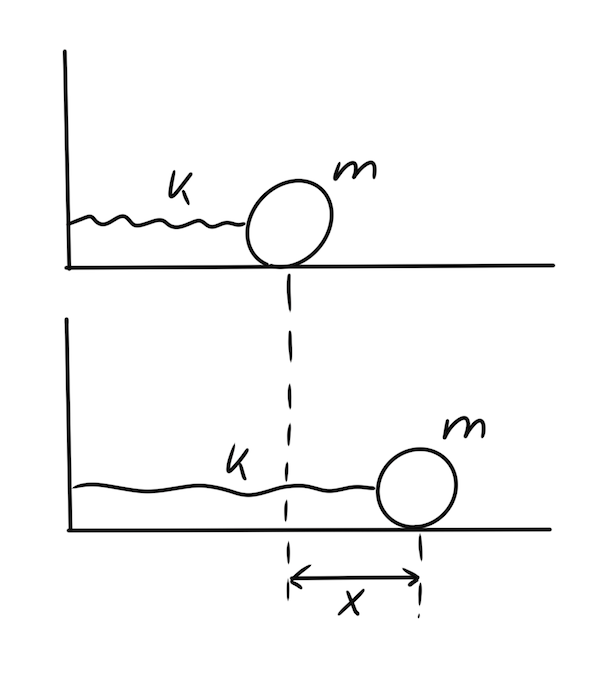
\includegraphics[width=0.3\textwidth]{/Users/vladbelousov/Desktop/Semestr_4-FP-NSU/ДфУ/Лекции_по_дням/image/17.png}
\end{center}

\[ T = \frac{m \dot{x } ^2 }{2} \quad  U = \frac{k x ^2 }{2}  \] 

\[ S = \int_{t_0 }^{t_1} \left( \frac{m \dot{x } ^2 }{2} -  \frac{k x ^2 }{2}\right)  dt \] 

Уравнение Эйлера (уравнение Лагранжа): \( \displaystyle  \frac{\partial L }{ \partial x  } - \frac{d}{dt} \frac{\partial L }{ \partial \dot{x}  } = 0  \) 

\[ - kx - \frac{d}{dt } ( m \dot{x } ) = 0  \Rightarrow m \ddot{x} + kx = 0  \] 

Понижение порядка: \( \displaystyle  L - \dot{x } \frac{\partial L}{\partial  \dot{x} } = C  \) 

\[ \frac{m \dot{x }  ^2 }{2 } - \frac{k x ^2 }{2 } - \dot{x } m \dot{x } = c \Rightarrow -\frac{m \dot{ x } ^2 }{2 } - \frac{k x ^2  }{2}  =c  - \text{ З.С.Э.}   \] 

\section{Изопериметрическая задача }

Найти кривую заданной длины, ограничивающую наибольшую площадь.

\[ \begin{aligned}
    S &\to  \max  \\ 
    l &= \mathrm{const}  
\end{aligned} \] 

\begin{center}
    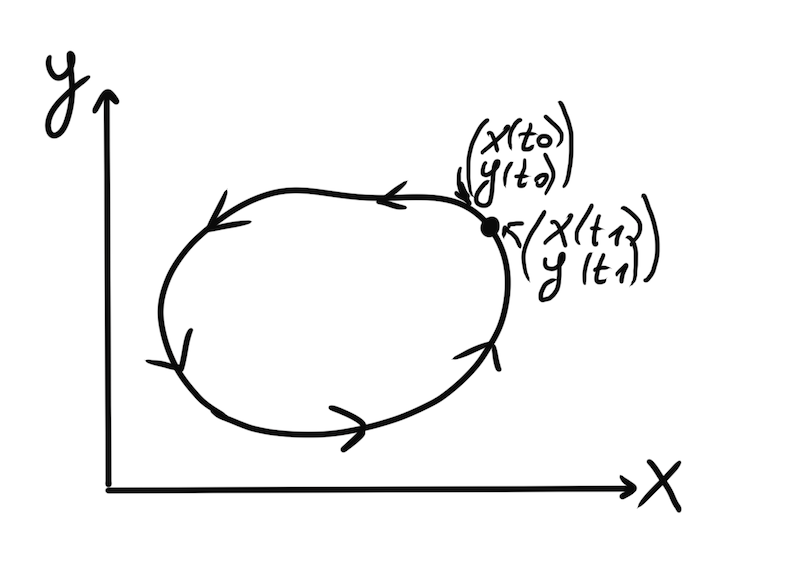
\includegraphics[width=0.5\textwidth]{/Users/vladbelousov/Desktop/Semestr_4-FP-NSU/ДфУ/Лекции_по_дням/image/18.png}
\end{center}

\[\begin{aligned}
    \begin{cases}
        x = x(t) \\ 
        y = y(t) \quad  t \in [ t_0 ,t_1]
        \end{cases}
    \begin{aligned}
        x(t_0 )=x(t_1) \\ 
        y(t_0 )=y(t_1) \\  
    \end{aligned}
\end{aligned} \]

\[ S = \iint_D dx dy   \] 

\[\text{ Формула Грина: }  \int_{ \partial D} \left( P(x,y )dx +Q(x,y )dy  \right) =\iint _D \left( - \frac{\partial P }{ \partial  y } (x,y ) + \frac{\partial Q}{\partial x }(x,y)   \right) dx dy\] 

\[ S = \iint_D dx dy = \iint_D \left(\underbrace{ \frac{1}{2 }}_{- \frac{\partial  P}{\partial y} } + \underbrace{ \frac{1}{2 }}_{ \frac{\partial  Q}{\partial x} }       \right)dx dy = \int_{ \partial  D } \left(  - \frac{y}{2 } dx + \frac{x}{2 } dy \right)  =\frac{1}{2 } \int_{t_0 }^{t_1} (x(t )y ' (t )- x' (t )y (t))dt  \] 

\[ \begin{cases}
\displaystyle \frac{\partial P } {\partial y } = -\frac{1}{2 }  \quad   P = - \frac{y}{2}  \\
\displaystyle \frac{\partial Q }{\partial x } = \frac{1}{2 } \quad  Q = \frac{x}{2}   
\end{cases} \] 

\[ l = \int_{t_0 }^{t_1} \sqrt{(x' (t ) ^2 + (y '(t ) )^2 } dt = \mathrm{const}   \] 

Задача из математического анализа : 

\[ \begin{cases}
f(x_1, \ldots, x_n ) \to  \mathrm{extz}   \quad \quad  \tilde{f } =f + \lambda_1 g_1 + ... + \lambda_m g_m \to  \mathrm{extz}   \\
g_1 (x_1, \ldots, x_n ) = 0 \\
\vdots \\
g_m (x_1, \ldots, x_n ) = 0
\end{cases} \] 

Задача вариационного исчисления: 

\[ I[y_1, \ldots, yn] = \int_{x_0 }^{x_1 } F(x,y_1, \ldots, y_n,y_1',..., y_n') dx \to  \mathrm{extz}   \] 

\[ \begin{cases}
y_1(x_0 ) = y_0 ^1 \quad  y_n(x_0 ) = y_0 ^n \\
y_1(x_1 ) = y_1 ^1 \quad  y_n(x_1 ) = y_1 ^n \\
\end{cases} \] 

\[ Y[y_1, \ldots, y_n ] = \int_{x_0 }^{x_1} G(x,y_1, \ldots, y_n,y_1',..., y_n')dx = \mathrm{const}    \] 

\textbf{Необходимое условие локального экстремума:} 

Пусть \( \tilde{y_1 }(x ),..., \tilde{y_n}(x) \) доставляет локальный экстремум функционалу \( I[y_1, \ldots, y_n] \)  и не является экстремалью функционалу \( Y[y_1, \ldots, y_n] \), тогда \( \exists  \lambda \in  \mathbb{R} \), такие, что \( \tilde{y_1}(x),..., \tilde{y_n}(x) \) доставляют экстремум функционалу \( \tilde{I } = I = \lambda Y \) 

\textbf{Без доказательства}

Замечание. \( I + \lambda Y \to  \mathrm{extz}  \Leftarrow \begin{cases}
    Y   = \mathrm{const}  \\
    I\to  \mathrm{extz} 
    \end{cases}  \) 

\[ \lambda \left( \frac{1}{\lambda }I + Y   \right) \to  \mathrm{extz} \Leftrightarrow Y+ \frac{1}{\lambda } \to  \mathrm{extz}  \Leftarrow \begin{cases}
Y \to  \mathrm{extz}  \\
I = \mathrm{const}  
\end{cases} \] 

Двойственная  задача: 

\[ \begin{aligned}
\begin{cases}
S \to  \max  \\
l = \mathrm{const}
\end{cases}
\Leftrightarrow 
\begin{cases}
l \to  \min  \\
S = \mathrm{const}
\end{cases}
\end{aligned} \]

\section{Решение классической изопериметрической задачи}

\[ \tilde{I } = S + \lambda l = \int_{t_0 }^{t_1 } \underbrace{\left[ \frac{1}{2 } (x y ' - x' y )+ \lambda \sqrt{(x') ^2 + (y ' ) ^2 } \right]}_{F}dt \to  \mathrm{extz}  \] 

\[ \begin{aligned}
    \begin{cases}
        \displaystyle \frac{\partial F }{\partial x } - \frac{d}{dt } \frac{\partial  F }{\partial  x ' } = 0 \quad  \\ 
        \vspace{0.01 mm} \\
        \displaystyle \frac{\partial F }{\partial y } - \frac{d}{dt } \frac{\partial  F }{\partial  y ' } = 0 \quad 
    \end{cases}
    \begin{cases}
        \displaystyle  \frac{1}{2 } y ' - \frac{d}{dt } \left[ -\frac{1}{2 } y + \lambda \frac{x ' }{\sqrt{(x') ^2 + (y ' ) ^2 }}  \right] =0\\
        \displaystyle -\frac{1}{2 } x ' - \frac{d}{dt } \left[ \frac{1}{2 } x + \lambda \frac{x ' }{\sqrt{(y') ^2 + (y ' ) ^2 }}  \right] =0 
    \end{cases}
\end{aligned}
\] 

№ 39 (задачник Александрова-Егорова).  Понизить порядок не получится так же, как в простейшей задаче.

\[ \begin{aligned}
    \begin{cases}
        \displaystyle \frac{d}{dt } \left[ \frac{y}{2 } + \frac{y}{2 } - \lambda \frac{x' }{\sqrt{(y') ^2 + (y ' ) ^2 }}  \right] =0 \\
        \displaystyle -\frac{d}{dt } \left[ \frac{x}{2 } + \frac{x}{2 } + \lambda \frac{y' }{\sqrt{(x') ^2 + (y ' ) ^2 }}  \right] =0
    \end{cases} 
    \begin{cases}
    \displaystyle y - c_1 = \frac{\lambda x' }{\sqrt{(x') ^2 + (y ' ) ^2 }} \\
    \displaystyle x - c_2 = \frac{-\lambda y' }{\sqrt{(x') ^2 + (y ' ) ^2 }}
    \end{cases}
\end{aligned}\] 

\[ \displaystyle (y- c_1 ) ^2 + (x- c_2 ) ^2 = \lambda ^2 \left[ \frac{(x') ^2 }{(x') ^2 + (y ' ) ^2 } + \frac{(y') ^2 }{(x') ^2 + (y ' ) ^2 } \right]  \] 

\[ \displaystyle (y- c_1 ) ^2 + (x- c_2 ) ^2 = \lambda ^2 - \text{окружность}  \] 




%%-------------------------------%%

% Закрытие документа, если файл компилируется отдельно
\ifdefined\mainfile
    % Если это основной файл, не нужно заканчивать документ
\else
    \end{document}
\fi